\section{Đề ôn thi giữa kỳ 2 toán 10}
\subsection{Phần trắc nghiệm}
Câu trắc nghiệm nhiều phương án lựa chọn. Học sinh trả lời từ
câu 1 đến câu 12. Mỗi câu hỏi học sinh \textit{chỉ chọn một} phương án.

\Opensolutionfile{ans}[Ans/Dapan]
 
\hienthiloigiaiex
%%%=============EX_1=============%%%
\begin{ex}%[0D7N1-1]%[Dự án đề kiểm tra Toán khối 10 GHKII NH23-24-Dot 2-Nguyễn Văn Nghĩa]%[Deso 10-CTST]
	Tam thức bậc hai nào sau đây luôn nhận giá trị dương trên khoảng $(1;3)$?
	\choice
	{$x^2-2 x-3$}
	{$x^2-3x+2$}
	{\True $x^2-2x+2$}
	{$x^2-4x+3$}
	\loigiai{
		Ta có $x^2-2x+2>0\,\forall x\in\mathbb{R}$ nên $x^2-2x+2$ nhận giá trị dương trên $(1;3)$.
		}
\end{ex}
%%%=============EX_2=============%%%
\begin{ex}%[0D7H2-6]%[Dự án đề kiểm tra Toán khối 10 GHKII NH23-24-Dot 2-Nguyễn Văn Nghĩa]%[Deso 10-CTST]
	Tam thức $f(x)=x^2-(m+2)x+5 m+1$ không âm với mọi $x$ khi?
	\choice
	{$m>16$}
	{\True $0\leq m\leq16$}
	{$m<16$}
	{$0<m<16$}
	\loigiai{
	Tam thức $f(x)=x^2-(m+2)x+5 m+1$ không âm với mọi $x$ thì $\heva{&a>0\\&\Delta\leq0}\Leftrightarrow\left(m+2\right)^2-4\cdot\left(5m+1\right)\leq0\Leftrightarrow m^2-16m\leq 0\Leftrightarrow 0\leq m\leq16$.
		}
\end{ex}
  
%%%=============EX_3=============%%%
 \begin{ex}%[0D7H2-6]%[Dự án đề kiểm tra Toán khối 10 GHKII NH23-24-Dot 2-Nguyễn Văn Nghĩa]%[Deso 10-CTST]
 	Giá trị của tham số $m$ để $x^2-2(m-1) x+m^2-2 m=0$ có hai nghiệm trái dấu, trong đó nghiệm âm có trị tuyệt đối lớn hơn nghiệm còn lại?
 	\choice
 	{$0<m<2$}
 	{\True $0<m<1$}
 	{$1<m<2$}
 	{$\hoac{&m>1\\&m<0}$}
 	\loigiai{
 	Để phương trình có $2$ nghiệm trái dấu thì $m^2-2m<0\Rightarrow0<m<2$.\\
 	Phương trình có $2$ nghiệm là $x_1=m$ và $x_2=m-2$.\\
 	Ta có $|x_1|<|x_2|\Rightarrow\left(x_1^2-x_2^2\right)<0\Rightarrow\left(x_1+x_2\right)<0\Rightarrow m<1$.\\
 	Vậy $0<m<1$.	
 	}
 \end{ex} 
  
%%%=============EX_4=============%%%
\begin{ex}%[0D7H3-1]%[Dự án đề kiểm tra Toán khối 10 GHKII NH23-24-Dot 2-Nguyễn Văn Nghĩa]%[Deso 10-CTST]
	Tập nghiệm của phương trình $\sqrt{x^2-3 x+1}=\sqrt{x-2}$ là
	\choice
	{$\left\{1;3\right\}$}
	{\True $\left\{3\right\}$}
	{$\left\{1\right\}$}
	{$\left\{3;6\right\}$}
	\loigiai{
	Bình phương $2$ vế phương trình ta được $x^2-3 x+1=x-2\Rightarrow\hoac{&x=1\\&x=3.}$\\
	Thay từng nghiệm vào phương trình ta thấy $x=3$ thỏa mãn.	
	}
\end{ex}   
  
%%%=============EX_5=============%%%
\begin{ex}%[0D7H3-1]%[Dự án đề kiểm tra Toán khối 10 GHKII NH23-24-Dot 2-Nguyễn Văn Nghĩa]%[Deso 10-CTST]
	Tập nghiệm của phương trình $\sqrt{x^2-x-2}=\sqrt{2x^2+x-1}$ là
	\choice
	{$\left\{3\right\}$}
	{$\left\{-1;2\right\}$}
	{$\left\{1\right\}$}
	{\True $\left\{-1\right\}$}
	\loigiai{
	Bình phương $2$ vế phương trình ta được $x^2-x-2=2x^2+x-1\\
	\Leftrightarrow x^2+2x+1=0\Rightarrow x=-1$.\\
	Với $x=-1$ thỏa mãn phương trình. 	
	}
\end{ex}    

%%%=============EX_6=============%%%
\begin{ex}%[0H9H2-1]%[Dự án đề kiểm tra Toán khối 10 GHKII NH23-24-Dot 2-Nguyễn Văn Nghĩa]%[Deso 10-CTST]
	Trong mặt phẳng tọa độ $Oxy$, cho hai điểm $A\left(3;1\right)$, $B\left(2;-6\right)$. Điểm $M$ thuộc trục hoành và $\widehat{ABM}=90^\circ$. Tọa độ điểm $M$ là 
	\choice
	{$(40;0)$}
	{$(0 ;-40)$}
	{\True $(-40 ; 0)$}
	{$(0 ; 40)$}
	\loigiai{
	Vì $M\in Ox$ nên $M\left(a;0\right)$.\\
	Ta có $\widehat{ABM}=90^\circ\Rightarrow\overrightarrow{BA}\perp \overrightarrow{BM}\Rightarrow \overrightarrow{BA}\cdot\overrightarrow{BM}=0$.\\
	Với $\heva{&\overrightarrow{BA}=\left(1;7\right)\\&\overrightarrow{BM}=\left(a-2;6\right)}\Rightarrow a-2+42=0\Rightarrow a=-40$.	
	}
\end{ex}   
  
%%%=============EX_7=============%%%
\begin{ex}%[0H5N1-1]%[Dự án đề kiểm tra Toán khối 10 GHKII NH23-24-Dot 2-Nguyễn Văn Nghĩa]%[Deso 10-CTST]
	Trong mặt phẳng tọa độ $Oxy$ cho vectơ $\overrightarrow{u}=(-2;3)$. Đẳng thức nào sau đây là đúng?
	\choice
	{$\overrightarrow{u}=2 \overrightarrow{i}+3 \overrightarrow{j}$}
	{$\overrightarrow{u}=3 \overrightarrow{i}+2 \overrightarrow{j}$}
	{\True $\overrightarrow{u}=-2 \overrightarrow{i}+3 \overrightarrow{j}$}
	{$\overrightarrow{u}=-2 \overrightarrow{j}+3 \overrightarrow{i}$}
	\loigiai{
	Ta có $\overrightarrow{u}=(-2;3)\Rightarrow\overrightarrow{u}=-2 \overrightarrow{i}+3 \overrightarrow{j}$.
	}
	\end{ex}

%%%=============EX_8=============%%%
\begin{ex}%[0H5N1-1]%[Dự án đề kiểm tra Toán khối 10 GHKII NH23-24-Dot 2-Nguyễn Văn Nghĩa]%[Deso 10-CTST]
\immini{Trong mặt phẳng tọa độ $O x y$ cho vectơ $\overrightarrow{u}$ như hình bên. Toạ độ của vectơ $\overrightarrow{u}$ là
	\choice
	{\True $(-4;2)$}
	{$(4;2)$}
	{$(2;-4)$}
	{$(2;4)$}
	\loigiai{
		Ta có $\overrightarrow{u}=(-4;2)$.	
	}
}{	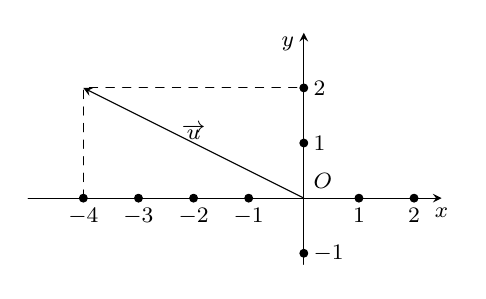
\begin{tikzpicture}[scale=0.7,font=\footnotesize,line join = round, line cap = round, >= stealth]
		\draw [->](-5,0)--(2.5,0);
		\draw [->](0,-1.2)--(0,3);
		\draw [->](0,0)--(-4,2);
		\draw (0,0) node[above right]{$O$} (0,1) node[right]{$1$} (0,2) node[right]{$2$} (0,-1) node[right]{$-1$} (-1,0) node[below]{$-1$} (-2,0) node[below]{$-2$} (-3,0) node[below]{$-3$} (-4,0) node[below]{$-4$} (1,0) node[below]{$1$} (2,0) node[below]{$2$}(2.5,0) node[below]{$x$}(0,2.8) node[left]{$y$} (-2,1.2) node{$\overrightarrow{u}$};
		\draw[dashed] (-4,0)--(-4,2)--(0,2);
		\draw[fill=black] 
		(0,1) circle (2pt) (0,2) circle (2pt) (-1,0) circle (2pt) (-2,0) circle (2pt) (-3,0) circle (2pt) (-4,0) circle (2pt) (0,-1) circle (2pt) (0,1) circle (2pt) (0,2) circle (2pt) (1,0) circle (2pt) (2,0) circle (2pt);
\end{tikzpicture}}	

\end{ex}

%%%=============EX_9=============%%%
\begin{ex}%[0H9N3-2]%[Dự án đề kiểm tra Toán khối 10 GHKII NH23-24-Dot 2-Nguyễn Văn Nghĩa]%[Deso 10-CTST]
	Phương trình đường thẳng đi qua hai điểm $A(-2;4)$, $B(-6;1)$ là
	\choice
	{$3x+4y-10=0$}
	{\True $3x-4y+22=0$}
	{$3x-4y+8=0$}
	{$3x-4y-22=0$}
	\loigiai{
	$\overrightarrow{AB}=\left(-4;-3\right)$ là vectơ chỉ phương của $AB$ nên $\overrightarrow{n}=\left(3;-4\right)$ là vectơ pháp tuyến của $AB$.\\
	Phương trình $\left(AB\right)\colon 3(x+2)-4(y-4)=0\Leftrightarrow 3x-4y+22=0$.	
	}
\end{ex}
  
%%%=============EX_10=============%%%
\begin{ex}%[0H9H2-2]%[Dự án đề kiểm tra Toán khối 10 GHKII NH23-24-Dot 2-Nguyễn Văn Nghĩa]%[Deso 10-CTST]
	Tìm côsin góc giữa hai đường thẳng $\mathrm{d}_1\colon10x+5y-1=0$ và $\mathrm{d}_2\colon\heva{&x=2+t\\&y=1-t.}$
	\choice
	{\True $\dfrac{3\sqrt{10}}{10}$}
	{$\dfrac{3}{5}$}
	{$\dfrac{\sqrt{10}}{10}$}
	{$\dfrac{3}{10}$}
	\loigiai{
	Ta có $\mathrm{d}_1\colon10x+5y-1=0\Rightarrow\overrightarrow{n_1}=\left(10;5\right)$ là vectơ pháp tuyến của $\mathrm{d}_1$.\\
	$\mathrm{d}_2:\heva{&x=2+t\\&y=1-t}\Rightarrow\overrightarrow{u_2}=\left(1;-1\right)$ là vectơ chỉ phương $\Rightarrow\overrightarrow{n_2}=\left(1;1\right)$ là vectơ pháp tuyến của $\mathrm{d}_2$.\\
	
	\begin{eqnarray*}
		&\cos\left(\mathrm{d}_1;\mathrm{d}_2\right) & =\dfrac{|\overrightarrow{n_1}\cdot\overrightarrow{n_2}|}{|\overrightarrow{n_1}||\overrightarrow{n_2}|}\\
		& & =\dfrac{|10\cdot1+5\cdot1|}{5\sqrt{5}\cdot\sqrt{2}}\\
		&& =\dfrac{3\sqrt{10}}{10}.
	\end{eqnarray*}	
	}
\end{ex}
  
%%%=============EX_11=============%%%
\begin{ex}%[0H9H4-2]%[Dự án đề kiểm tra Toán khối 10 GHKII NH23-24-Dot 2-Nguyễn Văn Nghĩa]%[Deso 10-CTST]
	Trong mặt phẳng tọa độ, cho tam giác $A B C$ có $A(1 ;-2), B(1 ; 2)$ và $C(5 ; 2)$. Phương trình đường tròn ngoại tiếp tam giác $A B C$ là
	\choice
	{$x^2+y^2-3 x+2 y+1=0$}
	{$x^2+y^2-3 x+1=0$}
	{$x^2+y^2-6 x-1=0$}
	{\True $x^2+y^2-6 x+1=0$}
	\loigiai{
	Gọi phương trình đường tròn có dạng $(\mathrm{C})\colon x^2+y^2-2ax-2by+c=0$.\\
	Vì $A,B,C\in(\mathrm{C})$.\\ 
	Ta có $\heva{&-2a+4b+c=-5\\&-2a-4b+c=-5\\&-10a-4b+c=-29}\Rightarrow\heva{&x=3\\&y=0\\&z=1.}$\\
	Vậy phương trình đường tròn là $(\mathrm{C})\colon x^2+y^2-6x+1=0$.	
	}
\end{ex}  
  
%%%=============EX_12=============%%%
\begin{ex}%[0H9N4-3]%[Dự án đề kiểm tra Toán khối 10 GHKII NH23-24-Dot 2-Nguyễn Văn Nghĩa]%[Deso 10-CTST]
	Phương trình tiếp tuyến của đường tròn $(\mathrm{C})\colon x^2+y^2-4 x+8y-5=0$ tại tiếp điểm $A(-1 ; 0)$ là
	\choice
	{$4 x+3 y+4=0$}
	{$3x+4y+3=0$}
	{\True $3x-4y+3=0$}
	{$-3x+y+22=0$}
	\loigiai{
	Ta có $I\left(2;-4\right)$ là tâm đường tròn.\\
	$\overrightarrow{IA}=\left(-3;4\right)$ là vectơ pháp tuyến của tiếp tuyến $\mathrm{d}$.\\
	$\left(\mathrm{d}\right)$ đi qua $A\left(-1;0\right)$ và có vectơ pháp tuyến $\overrightarrow{IA}=\left(-3;4\right)$.\\
	Phương trình $\mathrm{d}\colon -3x+4y-3=0\Rightarrow 3x-4y+3=0$.	
	}
\end{ex}

\Closesolutionfile{ans}
\bangdapan{Dapan}
\subsection{Câu trắc nghiệm đúng sai}
Học sinh trả lời từ câu 1 đến câu 4.
Trong mỗi ý \circlenum{A}, \circlenum{B}, \circlenum{C} và \circlenum{D} ở mỗi câu, học sinh chọn đúng hoặc sai.
\setcounter{ex}{0}
\LGexTF
\Opensolutionfile{ansbook}[ansbook/DapanDS]
\Opensolutionfile{ans}[Ans/DapanT]
\begin{ex}%[0D7H2-3]%[Dự án đề kiểm tra Toán khối 10 GHKIINH23-24-Dot2-ThinhNgo]%[Deso10-Sách CTST]
	Xét tính đúng sai của các khẳng định sau:
	\choiceTF
	{\True $f(x)=(2x-1)(3x^2-10x+3)$ có $f(x)<0$, $\forall x\in\left( -\infty; \dfrac{1}{3}\right) \cup \left( \dfrac{1}{2}; 3\right)$}
	{\True $f(x)=(-x^2+4)(2x^2-x-3)$ có $f(x)>0$, $\forall x\in\left( -2; -1\right) \cup \left( \dfrac{3}{2}; 2\right)$}
	{$f(x)=\dfrac{-x^2-2x}{(x-1)(x^2+1)}$ có $f(x)>0$, $\forall x\in\left( -2; 0\right) \cup \left( 1; +\infty\right)$}
	{$f(x)=\dfrac{x^3-6x^2+9x}{-2x^2+18}$ có $f(x)>0$, $\forall x\in\left( -3; 0\right) \cup \left(3; +\infty\right)$} 
	\loigiai{
		\begin{itemize}
			\item Xét $f(x)=0\Leftrightarrow (2x-1)(3x^2-10x+3)=0 \Leftrightarrow \hoac{& 2x-1=0 \\ & 3x^2-10x+3=0}\Leftrightarrow \hoac{& x=\dfrac{1}{2} \\ & x=\dfrac{1}{3}\vee x=3.}$\\
			Bảng xét dấu $f(x)$.
			\begin{center}
				\begin{tikzpicture}
					\tkzTabInit[deltacl=0.5,espcl=2.5,lgt=3]
					{$x$/1,$2x-1$/1,$3x^2-10x+3$/1,$f(x)$/1}
					{$-\infty$,$\dfrac{1}{3}$,$\dfrac{1}{2}$,$3$,$+\infty$}
					\tkzTabLine{,-,|,-,0,+,|,+,}
					\tkzTabLine{,+,0,-,|,-,0,+,}
					\tkzTabLine{,-,0,+,0,-,0,+,}
				\end{tikzpicture}	
			\end{center}
			Kết luận $f(x)<0 \Leftrightarrow \forall x\in\left( -\infty; \dfrac{1}{3}\right) \cup \left( \dfrac{1}{2}; 3\right)$.
			\item Xét $f(x)=0\Leftrightarrow (-x^2+4)(2x^2-x-3)=0 \Leftrightarrow \hoac{& -x^2+4=0 \\ & 2x^2-x-3=0}\Leftrightarrow \hoac{& x=2\vee x=-2 \\ & x=\dfrac{3}{2}\vee x=-1.}$\\
			Bảng xét dấu $f(x)$.
			\begin{center}
				\begin{tikzpicture}
					\tkzTabInit[deltacl=0.5,espcl=2.5,lgt=3]
					{$x$/1,$-x^2+4$/1,$2x^2-x-3$/1,$f(x)$/1}
					{$-\infty$,$-2$,$-1$,$\dfrac{3}{2}$,$2$,$+\infty$}
					\tkzTabLine{,-,0,+,|,+,|,+,0,-}
					\tkzTabLine{,+,|,+,0,-,0,+,|,+}
					\tkzTabLine{,-,0,+,0,-,0,+,0,-}
				\end{tikzpicture}		
			\end{center}
			Kết luận $f(x)>0 \Leftrightarrow \forall x\in\left( -2; -1\right) \cup \left( \dfrac{3}{2}; 2\right)$.
			\item Điều kiện $(x-1)(x^2+1)\neq 0 \Leftrightarrow \heva{& x-1\neq 0 \\ & x^2+1\neq 0}\Leftrightarrow \heva{& x\neq 1 \\ & \forall x\in \mathbb{R}}\Leftrightarrow x\neq 1$.\\
			Xét $f(x)=0\Leftrightarrow\dfrac{-x^2-2x}{(x-1)(x^2+1)}=0\Leftrightarrow -x^2-2x=0\Leftrightarrow x=0\vee x=-2$.\\
			Bảng xét dấu $f(x)$.
			\begin{center}
				\begin{tikzpicture}
					\tkzTabInit[deltacl=0.5,espcl=2.5,lgt=3]
					{$x$/1,$-x^2-2x$/1,$x-1$/1,$x^2+1$/1,$f(x)$/1}
					{$-\infty$,$-2$,$0$,$1$,$+\infty$}
					\tkzTabLine{,-,0,+,0,-,|,-,}
					\tkzTabLine{,-,|,-,|,-,0,+,}
					\tkzTabLine{,+,|,+,|,+,|,+,}
					\tkzTabLine{,+,0,-,0,+,d,-,}
				\end{tikzpicture}	
			\end{center}
			Kết luận $f(x)>0 \Leftrightarrow \forall x\in\left( -\infty; -2\right) \cup \left( 0; 1\right)$.
			\item Điều kiện $-2x^2+18\neq 0 \Leftrightarrow x^2\neq 9 \Leftrightarrow x\neq 3\vee x\neq -3$.\\
			Xét $f(x)=0\Leftrightarrow\dfrac{x^3-6x^2+9x}{-2x^2+18}=0\Leftrightarrow x(x-3)^2=0 \Leftrightarrow x=0\vee x=3$.\\
			Bảng xét dấu $f(x)$.
			\begin{center}
				
\begin{tikzpicture}
					\tkzTabInit[deltacl=0.5,espcl=2.5,lgt=3]
					{$x$/1,$x$/1,$(x-3)^2$/1,$-2x^2+18$/1,$f(x)$/1}
					{$-\infty$,$-3$,$0$,$3$,$+\infty$}
					\tkzTabLine{,-,|,-,0,+,|,+,}
					\tkzTabLine{,+,|,+,|,+,0,+,}
					\tkzTabLine{,+,0,+,|,+,0,+,}
					\tkzTabLine{,+,d,-,0,+,d,-,}
				\end{tikzpicture}	
			\end{center}
			Kết luận $f(x)>0 \Leftrightarrow \forall x\in\left( -\infty; -3\right) \cup \left(0; 3\right)$.
		\end{itemize}
	}
\end{ex}
\begin{ex}%[0D7H3-1]%[Dự án đề kiểm tra Toán khối 10 GHKIINH23-24-Dot2-ThinhNgo]%[Deso10-Sách CTST]
	Cho các phương trình sau $\sqrt{x^2-x-2}=\sqrt{-x^2+2x+3}$ ~ (1) và $\sqrt{x+2}=\sqrt{3x^2-x+1}$ ~ (2). Khi đó
	\choiceTF
	{\True Phương trình (1) có hai nghiệm phân biệt}
	{Phương trình (2) có một nghiệm}
	{\True Tổng các nghiệm của phương trình (1) bằng $\dfrac{3}{2}$}
	{\True Tổng các nghiệm của phương trình (2) bằng $\dfrac{2}{3}$}
	\loigiai{
		\begin{itemize}
			\item Bình phương hai vế của phương trình (1) ta có \\
			$x^2-x-2=-x^2+2x+3 \Leftrightarrow 2x^2-3x-5=0 \Leftrightarrow x=-1 \vee x= \dfrac{5}{2}$.\\
			Thay các giá trị $x=-1 \vee x= \dfrac{5}{2}$ vào phương trình (1), ta thấy chúng đều thỏa mãn.\\
			Vậy tập nghiệm của phương trình (1) là $S=\left\lbrace -1; \dfrac{5}{2}\right\rbrace $.
			\item Bình phương hai vế của phương trình (2) ta có \\
			$3x^2-x+1=x+2 \Leftrightarrow 3x^2-2x-1=0 \Leftrightarrow x=1 \vee x= -\dfrac{1}{3}$.\\
			Thay các giá trị $x=1 \vee x= -\dfrac{1}{3}$ vào phương trình (2), ta thấy chúng đều thỏa mãn.\\
			Vậy tập nghiệm của phương trình (2) là $S=\left\lbrace 1; -\dfrac{1}{3}\right\rbrace $.
			\item Theo cách giải ở trên ta có tổng các nghiệm của phương trình (1) bằng $\dfrac{3}{2}$.
			\item Theo cách giải ở trên ta có tổng các nghiệm của phương trình (2) bằng $\dfrac{2}{3}$.
		\end{itemize}
	}
\end{ex}

\begin{ex}%[0H9V3-7]%[Dự án đề kiểm tra Toán khối 10 GHKIINH23-24-Dot2-ThinhNgo]%[Deso10-Sách CTST]
	Trong mặt phẳng tọa độ $O x y$, cho hình chữ nhật $A B C D$ có tâm $I(6 ; 2)$ và các điểm $M(1 ; 5), $ $N(3 ; 4)$ lần lượt thuộc các đường thẳng $A B,$ $ B C$. Biết rằng trung điểm $E$ của cạnh $C D$ thuộc đường thẳng $\Delta\colon x+y-5=0$ và hoành độ của điểm $E$ nhỏ hơn 7. Khi đó
	\choiceTF
	{\True Phương trình $BC$ là $x-3=0$}
	{Phương trình $AB$ là $x+y-6=0$}
	{\True Tọa độ điểm $A$ là $A(9; 5)$}
	{Tọa độ điểm $B$ là $B(3; 3)$}
	\loigiai{
		\begin{center}
			\begin{tikzpicture}[scale=.7]
				\coordinate [label=above right:$B$](B) at (8,4);
				\coordinate [label=above left:$A$](A) at (0,4);
				\coordinate [label=below right:$C$](C) at (8,0);
				\coordinate [label=below left:$D$](D) at (0,0);
				\coordinate[label=above:$I$] (I) at ($(C)! .5 ! (A)$);
				\coordinate[label=below:$E$] (E) at ($(C)! .5 ! (D)$);
				\coordinate [label=above:$M$](M) at ($(A)! .7 ! (B)$);
				\coordinate [label=below:$P$](P) at ($(C)! .7 ! (D)$);
				\coordinate [label=right:$N$](N) at ($(B)! .2 ! (C)$);
				\foreach \diem in {A,B,C,D,E,M,P,I,N}	\fill (\diem)circle(1.5pt);		
				\draw[smooth](A)--(B)--(C)--(D)--(A)--(C) (B)--(D) (M)--(P);
				%	\draw[dashed];
				%	\foreach \x/\y/\z in {B/C/D}{\draw pic[draw,angle radius=2mm]{right angle=\x--\y--\z};}
			\end{tikzpicture}
		\end{center}
		Gọi $P$ đối xứng với $M(1; 5)$ qua $I(6; 2)$ suy ra $P(11 ;-1)$ và $P$ thuộc đường thẳng $C D$. \\Ta có $E$ thuộc $\Delta$ nên giả sử $E(t; 5-t)$. Khi đó $\overrightarrow{IE}=(t-6; 3-t), \overrightarrow{P E}=(t-11; 6-t)$.\\
		Vì $E$ là trung điểm $CD$ nên $I E \perp P E$. Do đó ta có
		\allowdisplaybreaks
		\begin{eqnarray*}
			\overrightarrow{IE} \cdot \overrightarrow{P E}=0 &\Leftrightarrow&(t-6)(t-11)+(3-t)(6-t)=0 \\&\Leftrightarrow& t^2-13 t+42=0\Leftrightarrow \hoac{&t=6\\&t=7.}
		\end{eqnarray*}
		Vì hoành độ của $E$ nhỏ hơn $7$ nên $E(6; -1)$ và .\\
		$BC$ đi qua $N(3; 4)$ và vuông góc với $PE$ nên $B C\colon x-3=0$.\\
		$AB$ đi qua $M(1; 5)$ và song song với $PE$ nên phương trình $AB\colon y-5=0$.\\
		Từ phương trình các cạnh tìm được ta có $A(9; 5), $ $B(3; 5)$, $ C(3;-1)$, $D(9; -1)$.}
\end{ex}
\begin{ex}%[0H9H4-4]%[0H9H4-3]%[0H9V4-2]%[Dự án đề kiểm tra Toán khối 10 GHKIINH23-24-Dot2-ThinhNgo]%[Deso10-Sách CTST]
	Cho đường tròn $(C)$ có phương trình $x^2+y^2-6 x+2 y+6=0$ và hai điểm $A(1 ;-1), $ $B(1 ; 3)$.
	Khi đó
	\choiceTF
	{\True Điểm $A$ thuộc đường tròn}
	{Điểm $B$ nằm trong đường tròn}
	{\True $x=1$ là phương trình tiếp tuyến của $(C)$ tại điểm $A$}
	{Qua $B$ kẻ được hai tiếp tuyến với $(C)$ có phương trình là $x=1; 3x+4y-12=0$}
	\loigiai{
		Đường tròn $(C)$ có tâm $I(3; -1)$ bán kính $R=\sqrt{9+1-6}=2$.
		\begin{itemize}
			\item Ta có $IA=2=R$ suy ra điểm $A$ thuộc đường tròn $(C)$.
			\item  $IB=2\sqrt{5}>R$ suy ra điểm $B$ nằm ngoài đường tròn $(C)$.
			\item Tiếp tuyến của $(C)$ tại điểm $A$ nhận $\overrightarrow{AI}=(2; 0)$ làm vec-tơ pháp tuyến nên có phương trình là $2(x-1)+0(y+1)=0$ hay $x=1$.
			\item Phương trình đường thẳng $\Delta$ đi qua $B$ có dạng $a(x-1)+b(y-3)=0$ (với $a^2+b^2 \neq 0$) hay $a x+b y-a-3 b=0$.\\
			Đường thẳng $\Delta$ là tiếp tuyến của đường tròn khi và chỉ khi 
			\allowdisplaybreaks
			\begin{eqnarray*}
				\mathrm{d} (I, \Delta)=R
				&\Leftrightarrow& \frac{|3 a-b-a-3 b|}{\sqrt{a^2+b^2}}=2 \Leftrightarrow(a-2 b)^2=a^2+b^2 \\&\Leftrightarrow& 3 b^2-4 a b=0 \Leftrightarrow \hoac{&b=0 \\&
					3 b=4 a.}
			\end{eqnarray*}
			\begin{itemize}
				\item Với $b=0$, chọn $a=1$; phương trình tiếp tuyến là $x=1$.
				\item Với $3 b=4 a$, chọn $a=3 \Rightarrow b=4$ phương trình tiếp tuyến là $3x+4y-15=0$.
			\end{itemize}
			Vậy qua $B$ kẻ được hai tiếp tuyến với $(C)$ có phương trình là $x=1 ;$ $ 3 x+4 y-15=0$.
			
	\end{itemize}}
\end{ex}
\Closesolutionfile{ans}
\Closesolutionfile{ansbook}

\begin{center}
	\textbf{\textsf{BẢNG ĐÁP ÁN ĐÚNG SAI}}
\end{center}
\input{Ansbook/DapanDS}

\subsection{Phần tự luận}

\hienthiloigiaibt
%%%=============BT_1=============%%%
\begin{bt}%[0D7V1-2]%[Dự án đề kiểm tra Toán khối 10 GHKIINH23-24-Dot2-Nguyen Cuong]%[Deso10-Sách CTST]
	Tìm tất cả các giá trị $m$ để bất phương trình $x^2+6x+m+7\le 0$ vô nghiệm.
	\loigiai{
		Bất phương trình $x^2+6x+m+7\le 0$ vô nghiệm khi và chỉ khi
		\allowdisplaybreaks
		\begin{eqnarray*}
			x^2+6x+m+7>0,\forall x\in\mathbb{R}&\Leftrightarrow&\heva{&a>0\\&\Delta'<0}\\
			&\Leftrightarrow&\heva{&1>0\\&3^2-m-7<0}\\
			&\Leftrightarrow& m>2.
		\end{eqnarray*}
		Vậy $m>2$ thì bất phương trình $x^2+6x+m+7\le 0$ vô nghiệm.
	}
\end{bt}
\begin{bt}%[0D7V1-2]%[Dự án đề kiểm tra Toán khối 10 GHKIINH23-24-Dot2-Nguyen Cuong]%[Deso10-Sách CTST]
	Tìm tất cả các giá trị $m$ để phương trình $(m-3)x^2+(m+3)x-(m+1)=0$ có hai nghiệm phân biệt.
	\loigiai{
		Phương trình có hai nghiệm phân biệt khi và chỉ khi
		\allowdisplaybreaks
		\begin{eqnarray*}
			\heva{&a\ne 0\\&\Delta >0}&\Leftrightarrow&\heva{&m-3\ne 0\\&(m+3)^2+4(m-3)(m+1)>0}\\
			&\Leftrightarrow&\heva{&m\ne 3\\&m^2+6m+9+4(m^2-2m-3)>0}\\
			&\Leftrightarrow&\heva{&m\ne 3\\&5m^2-2m-3>0}\\
			&\Leftrightarrow&\heva{&m\ne 3\\&m>1;m<-\dfrac{3}{5}.}
		\end{eqnarray*}
		Vậy $m\in \left(-\infty;-\dfrac{3}{5}\right)\cup (1;+\infty)\setminus\{3\}$.
	}
\end{bt}
\begin{bt}%[0D7C1-5]%[Dự án đề kiểm tra Toán khối 10 GHKIINH23-24-Dot2-Nguyen Cuong]%[Deso10-Sách CTST]
	Một công ty muốn làm một đường ống dẫn từ một điểm $A$ trên bờ đến một điểm $B$ trên một hòn đảo. Hòn đảo cách bờ biển $6$ km. Giá để xây đường ống trên bờ là $50\,000$ USD mỗi km, giá để xây đường ống dưới nước là $130\,000$ USD mỗi km; $B$ là điểm đến trên bờ sao cho $BB'$ vuông góc với bờ biển. Khoảng cách từ $A$ đến $B'$ là $9$ km. Biết rằng chi phí làm đường ống này là $1\,170\,000$ USD. Hỏi vị trí $C$ cách vị trí $A$ bao nhiêu km?
	\begin{center}
		\begin{tikzpicture}[join = round, cap = round, thick, font = \footnotesize, scale = 1]
			\path 
			(0:0) coordinate (B)++(-90:3) coordinate (B')++(0:3.5) coordinate (C)++(0:3) coordinate (A)
			;
			\draw 
			(B)--(B')node[midway,left]{$6$ km}
			(C)--(B')node[midway,below]{$x$ km}
			(C)--(A)node[midway,below]{$(9-x)$ km}
			(C)--(B)--(A)node[midway,above right]{biển}
			;
			\foreach \x/\g in {B/90,C/-90,B'/-90,A/-90}
			\fill (\x) circle (1.5pt)
			+(\g:3mm) node {$\x$};
		\end{tikzpicture}
	\end{center}
	\loigiai{
		Gọi $x=BC$ với $ 0\le x\le 9$, khi đó $BC=\sqrt{x^2+36}$.\\
		Số tiền xây dựng ống trên bờ là $50\,000(9-x)$.\\
		Số tiền xây dựng ống dưới nước là $130\,000\sqrt{x^2+36}$.\\
		Khi đó, ta có 
		\allowdisplaybreaks
		\begin{eqnarray*}
			50\,000(9-x)+130\,000\sqrt{x^2+36}=1\,170\,000&\Leftrightarrow&5(9-x)+13\sqrt{x^2+36}=117\\
			&\Leftrightarrow&13\sqrt{x^2+36}=5x+72\\
			&\Leftrightarrow&\heva{&5x+72\ge 0\\&169(x^2+36)=25x^2+720x+5184}\\
			&\Leftrightarrow&\heva{&x\ge-\dfrac{72}{5}\\&144x^2-720x+900=0}\\
			&\Leftrightarrow& x=\dfrac{5}{2}.
		\end{eqnarray*}
		Do đó $BC=2{,}5$ km và $AC=9-2{,}5=6{,}5$ km.\\
		Vậy vị trí điểm $C$ cách vị trí điểm $A$ một khoảng bằng $6{,}5$ km.
	}
\end{bt}
\begin{bt}%[0H9V2-6]%[Dự án đề kiểm tra Toán khối 10 GHKIINH23-24-Dot2-Nguyen Cuong]%[Deso10-Sách CTST]
	Trong mặt phẳng $Oxy$, cho ba điểm $A(-1;4)$, $B(1;1)$, $C(3;-1)$. Tìm điểm $N$ thuộc trục hoành sao cho $|NA-NC|$ bé nhất.
	\loigiai{
		Ta có $y_A\cdot y_C=4 \cdot(-1) < 0$ nên $A$, $C$ nằm khác phía so với trục $Ox$.\\
		Lấy điểm $C'$ đối xứng với $C$ qua $Ox$.\\
		Suy ra $C'(3; 1)$ và $C'$, $A$ cùng phía so với $Ox$.\\
		Ta có $N\in Ox \Rightarrow NC=NC'$.\\
		Vì vậy $|NA-NC|=\left|NA-NC'\right|\leq AC'$.\\
		Suy ra $|NA-NC|_{\max}=AC'$; giá trị lớn nhất này đạt được khi $A$, $C'$, $N$ thẳng hàng ($N$ nằm ngoài $A$, $C'$.\\
		Gọi $N(a; 0) \in Ox \Rightarrow \overrightarrow{AN}=(a+1;-4)$, $\overrightarrow{AC'}=(4;-3)$.\\
		Vì $\overrightarrow{AN}, \overrightarrow{AC'}$ cùng phương nên $\dfrac{a+1}{4}=\dfrac{-4}{-3} \Leftrightarrow-3 a-3=-16 \Leftrightarrow a=\dfrac{13}{3}$.\\
		Vậy $N\left(\dfrac{13}{3}; 0\right)$.
	}
\end{bt}
\begin{bt}%[0H9C3-6]%[Dự án đề kiểm tra Toán khối 10 GHKIINH23-24-Dot2-Nguyen Cuong]%[Deso10-Sách CTST]
	Trong mặt phẳng $Oxy$, cho hai điểm $A(1;6)$, $B(-3;4)$ và đường thẳng $\Delta\colon\heva{&x=1+t\\&y=1+2t}\, (t\in\mathbb{R})$. Tìm điểm $N$ thuộc đường thẳng $\Delta$ sao cho khoảng cách từ gốc tọa độ $O$ đến $N$ nhỏ nhất.
	\loigiai 
	{
		$N \in \Delta$ để $ON$ nhỏ nhất thì $ON \perp \Delta$.\\
		Ta có $N \in \Delta \Rightarrow N(1+t;1+2t)\Rightarrow \overrightarrow{ON}=(1+t;1+2t)$.\\	
		Véc-tơ chỉ phương của $\Delta$ là $\overrightarrow{u}_{\Delta}=(1;2)$.\\
		Vì $ON \perp \Delta \Rightarrow \overrightarrow{ON} \perp \overrightarrow{u}_{\Delta}$.\\
		Khi đó
		$$
		\overrightarrow{ON} \cdot \overrightarrow{u}_{\Delta}=0 \Leftrightarrow 1(1+t)+2(1+2 t)=0 \Leftrightarrow t=\frac{-3}{5}.
		$$
		Vậy $N\left(\dfrac{2}{5};\dfrac{-1}{5}\right)$.
	}
\end{bt}
\begin{bt}%[0H9C4-5]%[Dự án đề kiểm tra Toán khối 10 GHKIINH23-24-Dot2-Nguyen Cuong]%[Deso10-Sách CTST]
	Trong mặt phẳng $Oxy$, cho hai đường thẳng $d_1\colon x+3y+8=0$; $d_2\colon 3x-4y+10=0$ và điểm $A(-2;1)$. Viết phương trình đường tròn $(C)$ có tâm thuộc đường thẳng $d_1$, đi qua điểm $A$ và tiếp xúc với $d_2$.
	\loigiai
	{
		Gọi $I$ là tâm đường tròn $(C)$. Do $I\in d_1$ nên $I(-3a-8;a)$.\\
		Suy ra $\overrightarrow{AI}=(-3a-6;a-1)$ và $R=AI=\sqrt{(-3a-6)^2+(a-1)^2}=\sqrt{10a^2+34a+37}$.\\
		Đường tròn $(C)$ tiếp xúc với $d_2$ khi và chỉ khi
		\allowdisplaybreaks
		\begin{eqnarray*}
			\mathrm{d}(I;d_2)=AI&\Leftrightarrow&\dfrac{|3(-3a-8)-4a+10|}{\sqrt{3^2+(-4)^2}}=\sqrt{10a^2+34a+37}\\
			&\Leftrightarrow&|-13a-14|=5\sqrt{10a^2+34a+37}\\
			&\Leftrightarrow& (13a+14)^2=25(10a^2+34a+37)\\
			&\Leftrightarrow&169a^2+364a+196=250a^2+850a+925\\
			&\Leftrightarrow&81a^2+486a+729=0\\
			&\Leftrightarrow&a=-3.
		\end{eqnarray*}
		Suy ra tâm $I(1;-3)$ và $R=AI=5$.\\
		Vậy phương trình đường tròn $(C)\colon (x-1)^2+(y+3)^2=25$.
	}
\end{bt}
